\documentclass[a4paper,12pt]{article} % declaration

% packages

\usepackage[utf8]{inputenc}
\usepackage{amsmath}
\usepackage{amsthm}
\usepackage{amsfonts}
\usepackage{color}
\usepackage{graphicx}
\usepackage{tikz}

\newtheorem{definition}{Definition}[section]
\newtheorem{theorem}{Theorem}[section]
\newtheorem{proposition}{Proposition}[section]
\newtheorem{lemma}[theorem]{Lemma}
\newtheorem{corollary}[theorem]{Corollary}
\newtheorem{example}{Examples}
\newtheorem*{remark}{Remark}
\title{Derivative}
\author{Guoning Wu}
\begin{document}
\tableofcontents
\setcounter{tocdepth}{2}
\listoffigures
\listoftables
\maketitle
%======================================================
\section{Differentiable Functions}
\begin{definition}
    A function $f: E \to \mathbb{R}$ defined on a set $E$ is 
    differentiable at a point $a \in E$ that is a limit point 
    of $E$ if there exists a linear function $A(x-a)$  of 
    the increment $x-a$ of the argument such that $f(x) - f(a)$
    can be represented as 
    \begin{equation}
        f(x) - f(a) = A(x-a) + \circ(x-a) \text{ as } x \to a, a \in E
        \label{eq:eq1}
    \end{equation}
\end{definition}

In other words, a function is differentiable at a point $a$ if 
the change in its values in a neighborhood of the point in 
question is linear up to a correction that is infinitesimal 
compared with the magnitude of the displacement $x - a$
for the point $a$.

\begin{definition}
    The linear function $A(x-a)$ in Eq.~\ref{eq:eq1} is called 
    the differential of the function $f$ at $a$.
\end{definition}

The number $A$ is unambiguously determined due to the uniqueness 
of the limit.

\begin{definition}
    The number 
    \begin{equation}
        f'(a) = \lim_{x \to a} \frac{f(x)-f(a)}{x-a}
        \label{eq:eq2}
    \end{equation}
    is called the derivative of the function $f$ at $a$.
\end{definition}

Graphically, this definition says that the derivative of $f$ at 
$a$ is the slope of the tangent line to $y = f(x)$ at $a$,
which is the limit as $x \to a$ of the slopes of the lines 
through $(x,f(x))$ and $(a,f(a))$.

We can also write 
\[
    f'(a) = \lim_{\Delta x \to 0} \frac{f(a+\Delta x) - f(a)}{\Delta x}
    \]

\begin{definition}
    A function $f: E \to \mathbb{R}$ defined on a set $E \subset \mathbb{R}$
    is differentiable at a point $x \in E$ that is a limit point of $E$
    if 
    \begin{equation}
        f(x+h) - f(x) = A(x)h + \alpha(x;h)
        \label{eq:eq3}
    \end{equation}
    where $h \to A(x)h$ is a linear function in $h$ and $\alpha(x;h) = \circ(h)$
    as $h \to 0, x+h \in E$.
\end{definition}

\begin{definition}
    The function $h \to A(x)h$ of Definition~\ref{eq:eq3}, which 
    is linear in $h$, is called the differential of the function 
    $f: E \to \mathbb{R}$ at the point $x \in E$ and is denoted as 
    $df(x)$ or $Df(x)$.
\end{definition}

Thus, $df(x)(h) = A(x)h.$

From definitions \ref{eq:eq2} and \ref{eq:eq3} we have
\[
    \Delta f(x;h) - df(x)(h) = \alpha(x;h)
    \]
\subsection{Some Examples}

\begin{example}
    Let $f(x) = \sin x$. We shall show that $f'(x) = \cos x$.
\end{example}

\begin{example}
    We shall show that $\cos'(x) = - \sin x$.
\end{example}

\begin{example}
    If $f(t) = r\sin \omega t$, then $f'(t) = r\omega \cos \omega t.$
    If $f(t) = r\cos \omega t$, then $f'(t) = -r\omega \sin \omega t.$
\end{example}

\begin{example}
    The instantaneous velocity and instantaneous acceleration 
    of a point mass. Suppose a point mass is moving in a plane 
    and that in some given coordinate system its motion 
    is described by differentiable function of time 
    \[
        x = x(t), y=y(t)
    \]
    In particular, this motion is written as in the form 
    \[
        r(t) = \left(r\cos (\omega t + \alpha), r\sin (\omega t+ \alpha)\right)
    \]
\end{example}

\begin{example}
    The optic property of a parabolic mirror. Let us consider the 
    parabola $y = \frac{1}{2p}x^2(p>0)$, and construct the tangent to 
    it at the point $(x_0, y_0) = (x_0, \frac{1}{2p}x_0^2)$.  
\end{example}

\begin{example}
    \[
        f(x) = \left\{\begin{array}{c} x^2\sin \frac{1}{x}, \text{ if } x \ne 0 \\
        0, \text{ if } x = 0. \end{array} \right.
        \]
\end{example}

\begin{example}
    We shall show that 
    \[
        e^{x+h} - e^x = e^xh + \circ(h)
        \] as $h \to 0$.
\end{example}

\begin{example}
    If $a > 0$, then $a^{x+h} - a^x = a^h(\ln a)h + \circ(h)$
    as $h \to 0.$
\end{example}

\section{The Basic Rules of Differentiation}
\subsection{Differentiation and the Arithmetic Operations}
\begin{theorem}
    If function $f: X \to \mathbb{R}$ and $g: X \to \mathbb{R}$ are 
    differentiable at a point $x \in X$, then 
    a) their sum is differentiable at $x$, and 
    \[
        \left(f+g\right)'(x) = \left(f' + g'\right)(x),
        \]
    b) their product is differentiable at $x$, and 
    \[
        \left(f\cdot g\right)'(x) = f'(x)\cdot g(x) + f(x)\cdot g'(x),
        \]
    c) their quotient is differentiable at $x$ if $g(x) \ne 0$, and 
    \[
        \left(\frac{f}{g}\right)'(x) = \frac{f'(x)g(x) - f(x)g'(x)}{g^2(x)}.
        \]
\end{theorem}

\begin{corollary}
    The derivative of a linear combination of differentiable functions 
    equals the same linear combination of the derivatives of these 
    functions.
\end{corollary}

\begin{corollary}
    If the functions $f_1, \cdots, f_n$ are differentiable at $x$, then 
    \[
        \begin{split}
            \left(f_1f_2\cdots f_n\right)'(x) &= f_1'f_2\cdots f_n \\
            & + f_1f_2'\cdots f_n  + \cdots + f_1f_2\cdots f_n'
        \end{split}
        \]
\end{corollary}

\begin{corollary}
    It follows from the relation between the derivative and the 
    differential that we have:
    \[
        \begin{split}
            & a) d(f+g)(x) = df(x) + dg(x),\\
            & b) d(f\cdot g)(x) = g(x)df(x) + f(x)dg(x),\\
            & c) d\left(\frac{f}{g}\right)(x) = \frac{g(x)df(x) - f(x)dg(x)}{g^2(x)}.
        \end{split}
        \]
\end{corollary}

\begin{example}
    Find the derivative of $\displaystyle \tan x$ and 
    $\cot x$.
\end{example}

\subsection{Differentiation of a Composite Function (chain rule)}
\begin{theorem}
    If the function: $f: X \to Y \subset \mathbb{R}$  is differentiable 
    at a point $x \in X$ and the function $g: Y \to \mathbb{R}$
    is differentiable at the point $y = f(x) \in Y$, then the composite 
    function $g \circ f: X \to \mathbb{R}$ is differentiable at $x$, and the 
    differential $\rm{d} (g \circ f)(x): T\mathbb{R} \to T\mathbb{R}g(f(x))$
    of their composition equals the composition $\rm{d}g(y) \circ \rm{d}f(x)$ of 
    their differentials.
\end{theorem}

\begin{corollary}
    The derivative $(g \circ f)'(x)$ of the composition of differentiable 
    real-valued functions equals the product $g'(f(x)) \cdot f'(x)$ of the derivatives 
    of these functions computed at the corresponding points.
\end{corollary}

\[
    \frac{\Delta z}{\Delta x} = \frac{\Delta z}{\Delta y} \cdot \frac{\Delta y}{\Delta x}
    \]
\begin{example}
    Let us show that for $\alpha \in \mathbb{R}$ we have $\frac{\mathrm{d}x^{\alpha}}{\mathrm{d}x} 
    = \alpha x^{\alpha -1}$ in the domain $x > 0$, that is, $\mathrm{d} x^{\alpha}  = \alpha x^{\alpha - 1}\mathrm{d}x$
\end{example}

\begin{example}
    The derivative of the logarithm of the absolute value of a differentiable 
    function is often called its logarithmic derivative.
    \[
        \mathrm{d}\left(\ln |f|\right)(x) = \frac{f'(x)}{f(x)} \mathrm{d}x = \frac{\mathrm{d}f(x)}{f(x)}.
        \]
\end{example}

\begin{example}
    The absolute and relative errors in the value of a differentiable function caused by 
    errors in the data for the argument.
    \[
        f(x+h) - f(x) = f'(x)h + \alpha(x;h),
    \]
    \[
        \frac{|f'(x)h|}{|f(x)|} = \frac{|\mathrm{d}f(x)h|}{|f(x)|}
        \]
\end{example}

\subsection{Differentiation of an Inverse Function}
\begin{theorem}
    Let the function $f: X \to Y$ and $f^{-1}: Y \to X$ be mutually inverse and continuous 
    at points $x_0$ and $f(x_0) = y_0 \in Y$ respectively. If $f$ is differentiable at 
    $x_0$ and $f'(x_0) \ne 0$, then $f^{-1}$ is also differentiable at the point $y_0$, and 
    \[
        \left(f^{-1}\right)'(y_0) = \left(f'(x_0)\right)^{-1}.
        \]
\end{theorem}

\begin{remark}
    If we knew in advance that the function $f^{-1}$ was differentiable at $y_0$, we would find 
    immediately by the identity $\left(f^{-1} \circ f\right)(x) = x$ and the theorem on differentiation 
    of a composite function that $\left(f^{-1}\right)'\cdot f'(x_0) = 1.$
\end{remark}

\begin{remark}
    The condition $f'(x_0) \ne 0$ is obviously equivalent to the statement that the mapping 
    $h \to f'(x_0)h$ realized by the differential $\mathrm{d}f(x_0):
    T\mathbb{R}(x_0) \to T\mathbb{R}(y_0)$ is invertible mapping $\left[\mathrm{d}f(x_0)\right]^{-1}: T\mathbb{R}(y_0)
     \to T\mathbb{R}(x_0)$ given by the formula $ \tau \to \left(f'(x_0)\right)^{-1}\tau$.
\end{remark}

\begin{example}
    We shall show that $\arcsin'y = \frac{1}{1-y^2}$ for $|y| < 1$.
\end{example}

\begin{example}
    $\displaystyle arccot'y = -\frac{1}{1+y^2}, \arctan'y = \frac{1}{1+y^2}$
\end{example}

\begin{example}
    The hyperbolic and inverse hyperbolic functions and their derivatives.
    The function 
    \[
        \begin{split}
        \sinh x = \frac{1}{2}\left(e^x - e^{-x}\right) \\
        \cosh x = \frac{1}{2}\left(e^x - e^{-x}\right)
        \end{split}
        \]
    are respectively the hyperbolic sine and hyperbolic cosine of $x$.
    These functions, which for the time being have been introduced purely 
    formally, arise just as naturally in many problems as the circular 
    functions $\sin x$ and $\cos x$.

    We remark that 
    \[
        \begin{split}
            \sinh (-x) = -\sinh x \\
            \cosh (-x) =  \cosh x
        \end{split}
        \]
    Moreover, the following basic identity is obvious
    \[
        \cosh^2x - \sinh^2x = 1
        \]
    The graphs of the functions $y = \sinh x$ and $y = \cosh x$ are shown in 
    Fig~\ref{fig:hyps}. The inverse of the hyperbolic sine is 
    \[
        x = \ln (y + \sqrt{1+y^2})
        \]
    Thus, 
    \[
        \sinh^{-1} y = \ln(y + \sqrt{1+y^2})
        \]
    \graphicspath{
        {./Figs/}
    }
    \begin{figure}[htbp]
        \centering
        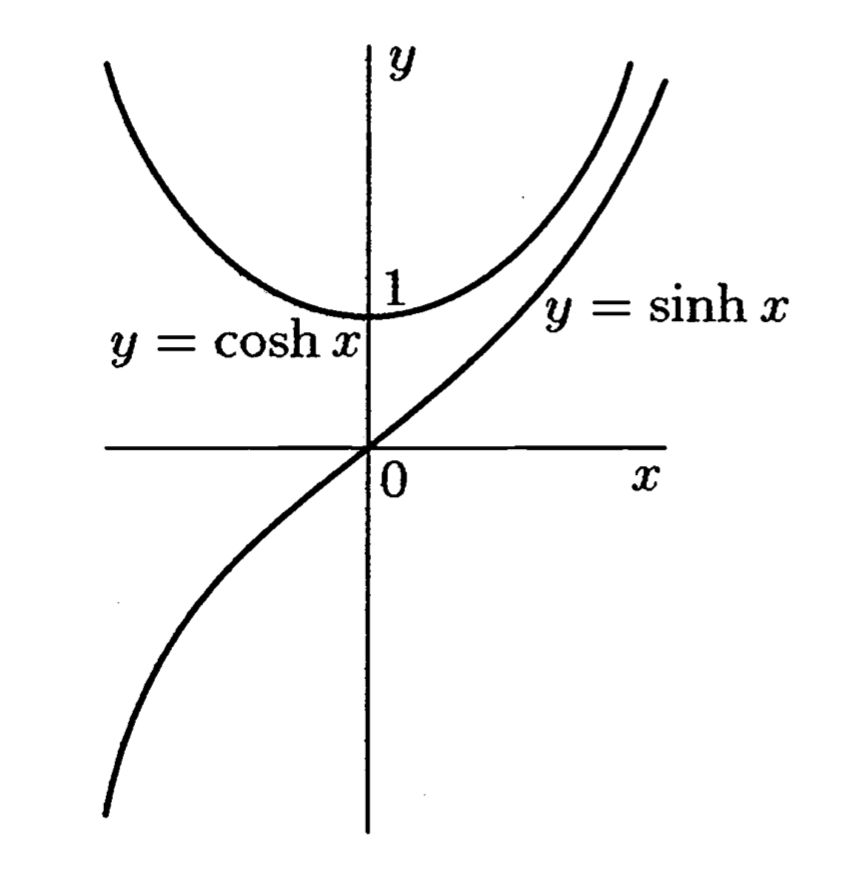
\includegraphics[width=0.5\textwidth]{hyps.png}
        \caption{Hyperbolic functions.}
        \label{fig:hyps}
    \end{figure}
    Similarly, using the monotonicity of the function $y = \cosh x$
    on its definition, we have 
    \[
        \begin{split}
            \cosh^{-1}_-(y) = \ln \left(y - \sqrt{y^2 - 1}\right)\\
            \cosh^{-1}_+(y) = \ln \left(y + \sqrt{y^2 - 1}\right)
        \end{split}
        \]
    From the definitions given above, we find 
    \[
        \begin{split}
            \sinh'x = \cosh x,\\
            \cosh'x = \sinh x,
        \end{split}
        \]
    and by the theorem on the derivative of an inverse function, we find
    \[
        \begin{split}
            \left(\sinh^{-1}y\right)' = \frac{1}{\sinh'x} = \frac{1}{\cosh'x} = \frac{1}{\sqrt{1+y^2}}\\
            \left(\cosh_-^{-1}y\right)' = \frac{1}{\cosh'x} = \frac{1}{\cosh'x} = \frac{1}{-\sqrt{\cosh^2x-1}} = -\frac{1}{\sqrt{y^2-1}}, y > 1\\
            \left(\cosh_+^{-1}y\right)' = \frac{1}{\cosh'x} = \frac{1}{-\sqrt{\cosh^2x-1}} = -\frac{1}{\sqrt{y^2-1}}, y > 1
        \end{split}
        \]
    Like $\tan x$ and $\cot x$ one can consider the functions 
    \[
        \tanh x = \frac{\sinh x}{\cosh x}, and \coth x = \frac{\cosh x}{\sinh x}
        \]
    called the hyperbolic tangent and hyperbolic cotangent respectively, and also 
    the functions inverse to them, the area tangent 
    \[
        \begin{split}
        \tanh^{-1} y = \frac{1}{2}\ln\frac{1+y}{1-y}, |y| < 1,
        \coth^{-1} y = \frac{1}{2}\ln\frac{y+1}{y-1}, |y| > 1,
        \end{split}
        \]
    By the rules for differentiation we have 
    \[
        \begin{split}
            \tanh'x = \frac{1}{\cosh^2x}\\
            \coth'x = -\frac{1}{\sinh x}
        \end{split}
        \]
    By the theorem on the derivative of an inverse function 

\end{example}
\section{Table of Derivatives of the Basic Elementary Functions}
\graphicspath{
        {./Figs/}
}
\begin{figure}[htbp]
        \centering
        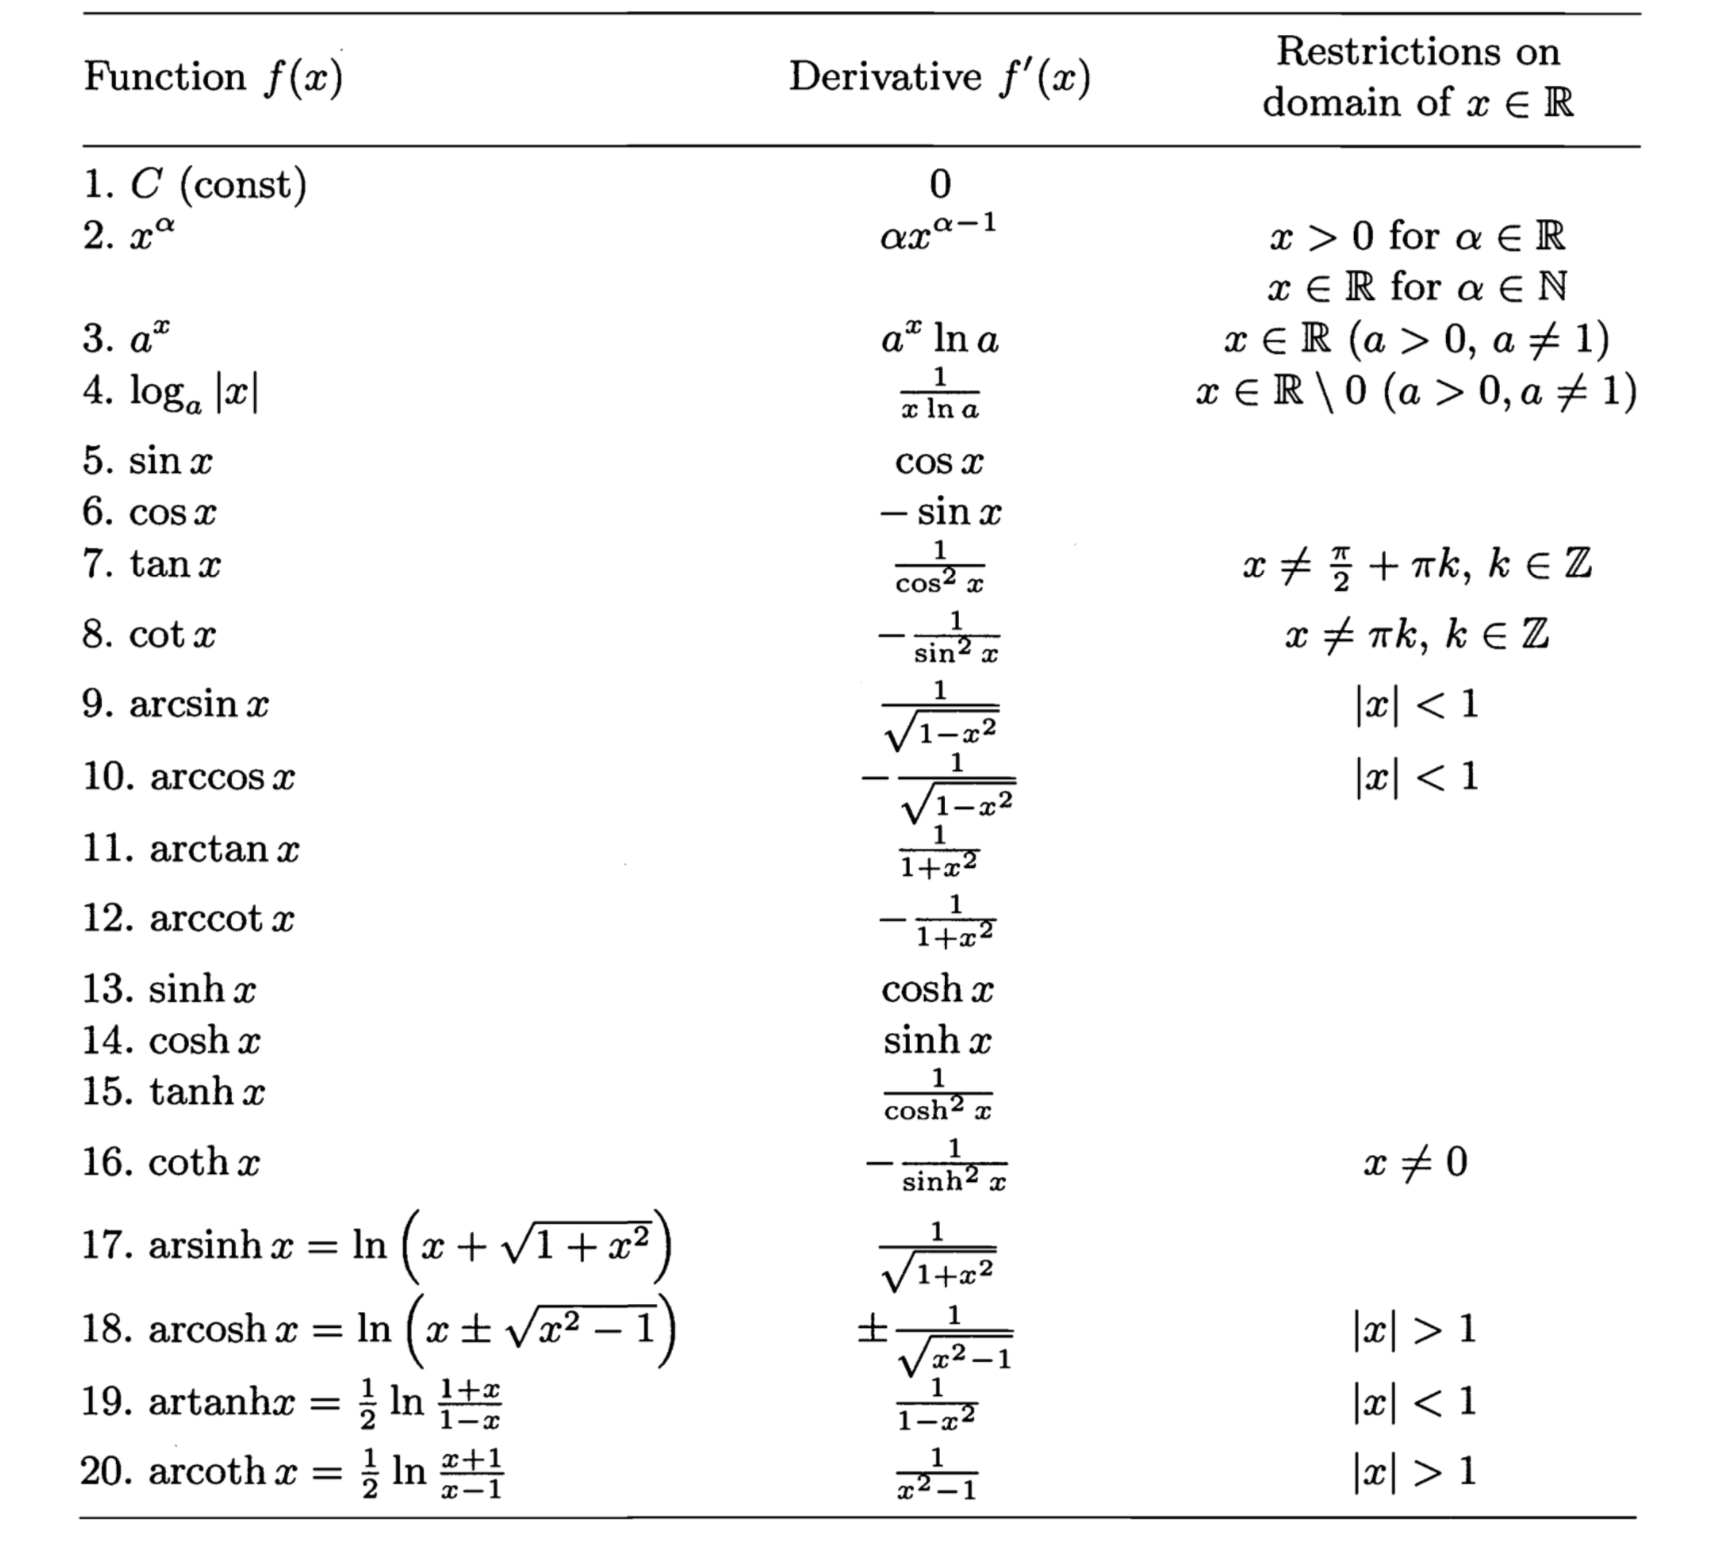
\includegraphics[width=0.9\textwidth,height=1.2\textwidth]{tableofderi.png}
        \caption{Table of Derivatives of the Basic Elementary Functions.}
        \label{fig:hyps}
\end{figure}

\section{Higher-order Drivative}
If a function $f: E \to \mathbb{R}$ is differentiable at every point $x \in E$,
then a new function $f': E \to \mathbb{R}$ arises, whose value at a point 
$x \in E$ equals the derivative $f'(x)$ of the function $f$ at that point.

The function $f': E \to \mathbb{R}$ may itself has a derivative $$

\end{document}
